\section{Einstein Coefficients}

Einstein coefficients express the probability of emission/absorption of light by an atom/molecule. The A coefficients tells us about the rate of spontaneous emission of light, and the Bs about absorption and stimulated emission of light. Anytime we are talking about emission, we use the index $ul$, which means that the electron moved from a more energetic state to a lower one, allowing then the emission of a photon. When referring to an absorption, we use the index $lu$, which means the opposite: electron getting more energetic and moving up to a higher state due to the absorption of a photon. Following this, we have the following Einstein coefficients:
\\
\\$B_{lu}$ = Einstein absorption [$s^{-1}\;erg^{-1}\;cm^2\;str$]
\\$B_{ul} =$ Einstein stimulated emission [$s^{-1}\;erg^{-1}\;cm^2\;str$]
\\$A_{ul} =$ Einstein spontaneous emission [$s^{-1}$]
\\
\\We can relate those coefficients as expressed below:
\\
\\$g_lB_{lu} = g_u B_{ul}$
\\
\\$B_{ul} = \frac{c^3}{8\pi h \nu^3}$
\\
\\$B_{lu} = \frac{g_u}{g_l} \frac{c^3}{8\pi h \nu^3} A_{ul}$


The intensity for a determined frequency $\nu$ is
\\$B_{\nu} = \frac{\frac{A_{ul}}{B_{ul}}}{\frac{g_l B_{lu}}{g_u B_{ul}} \exp{(\frac{h\nu}{KT})}-1}$

Also:
\\$\frac{n_l}{n_u} = \frac{g_l}{g_u}e^{h\nu/kT}$


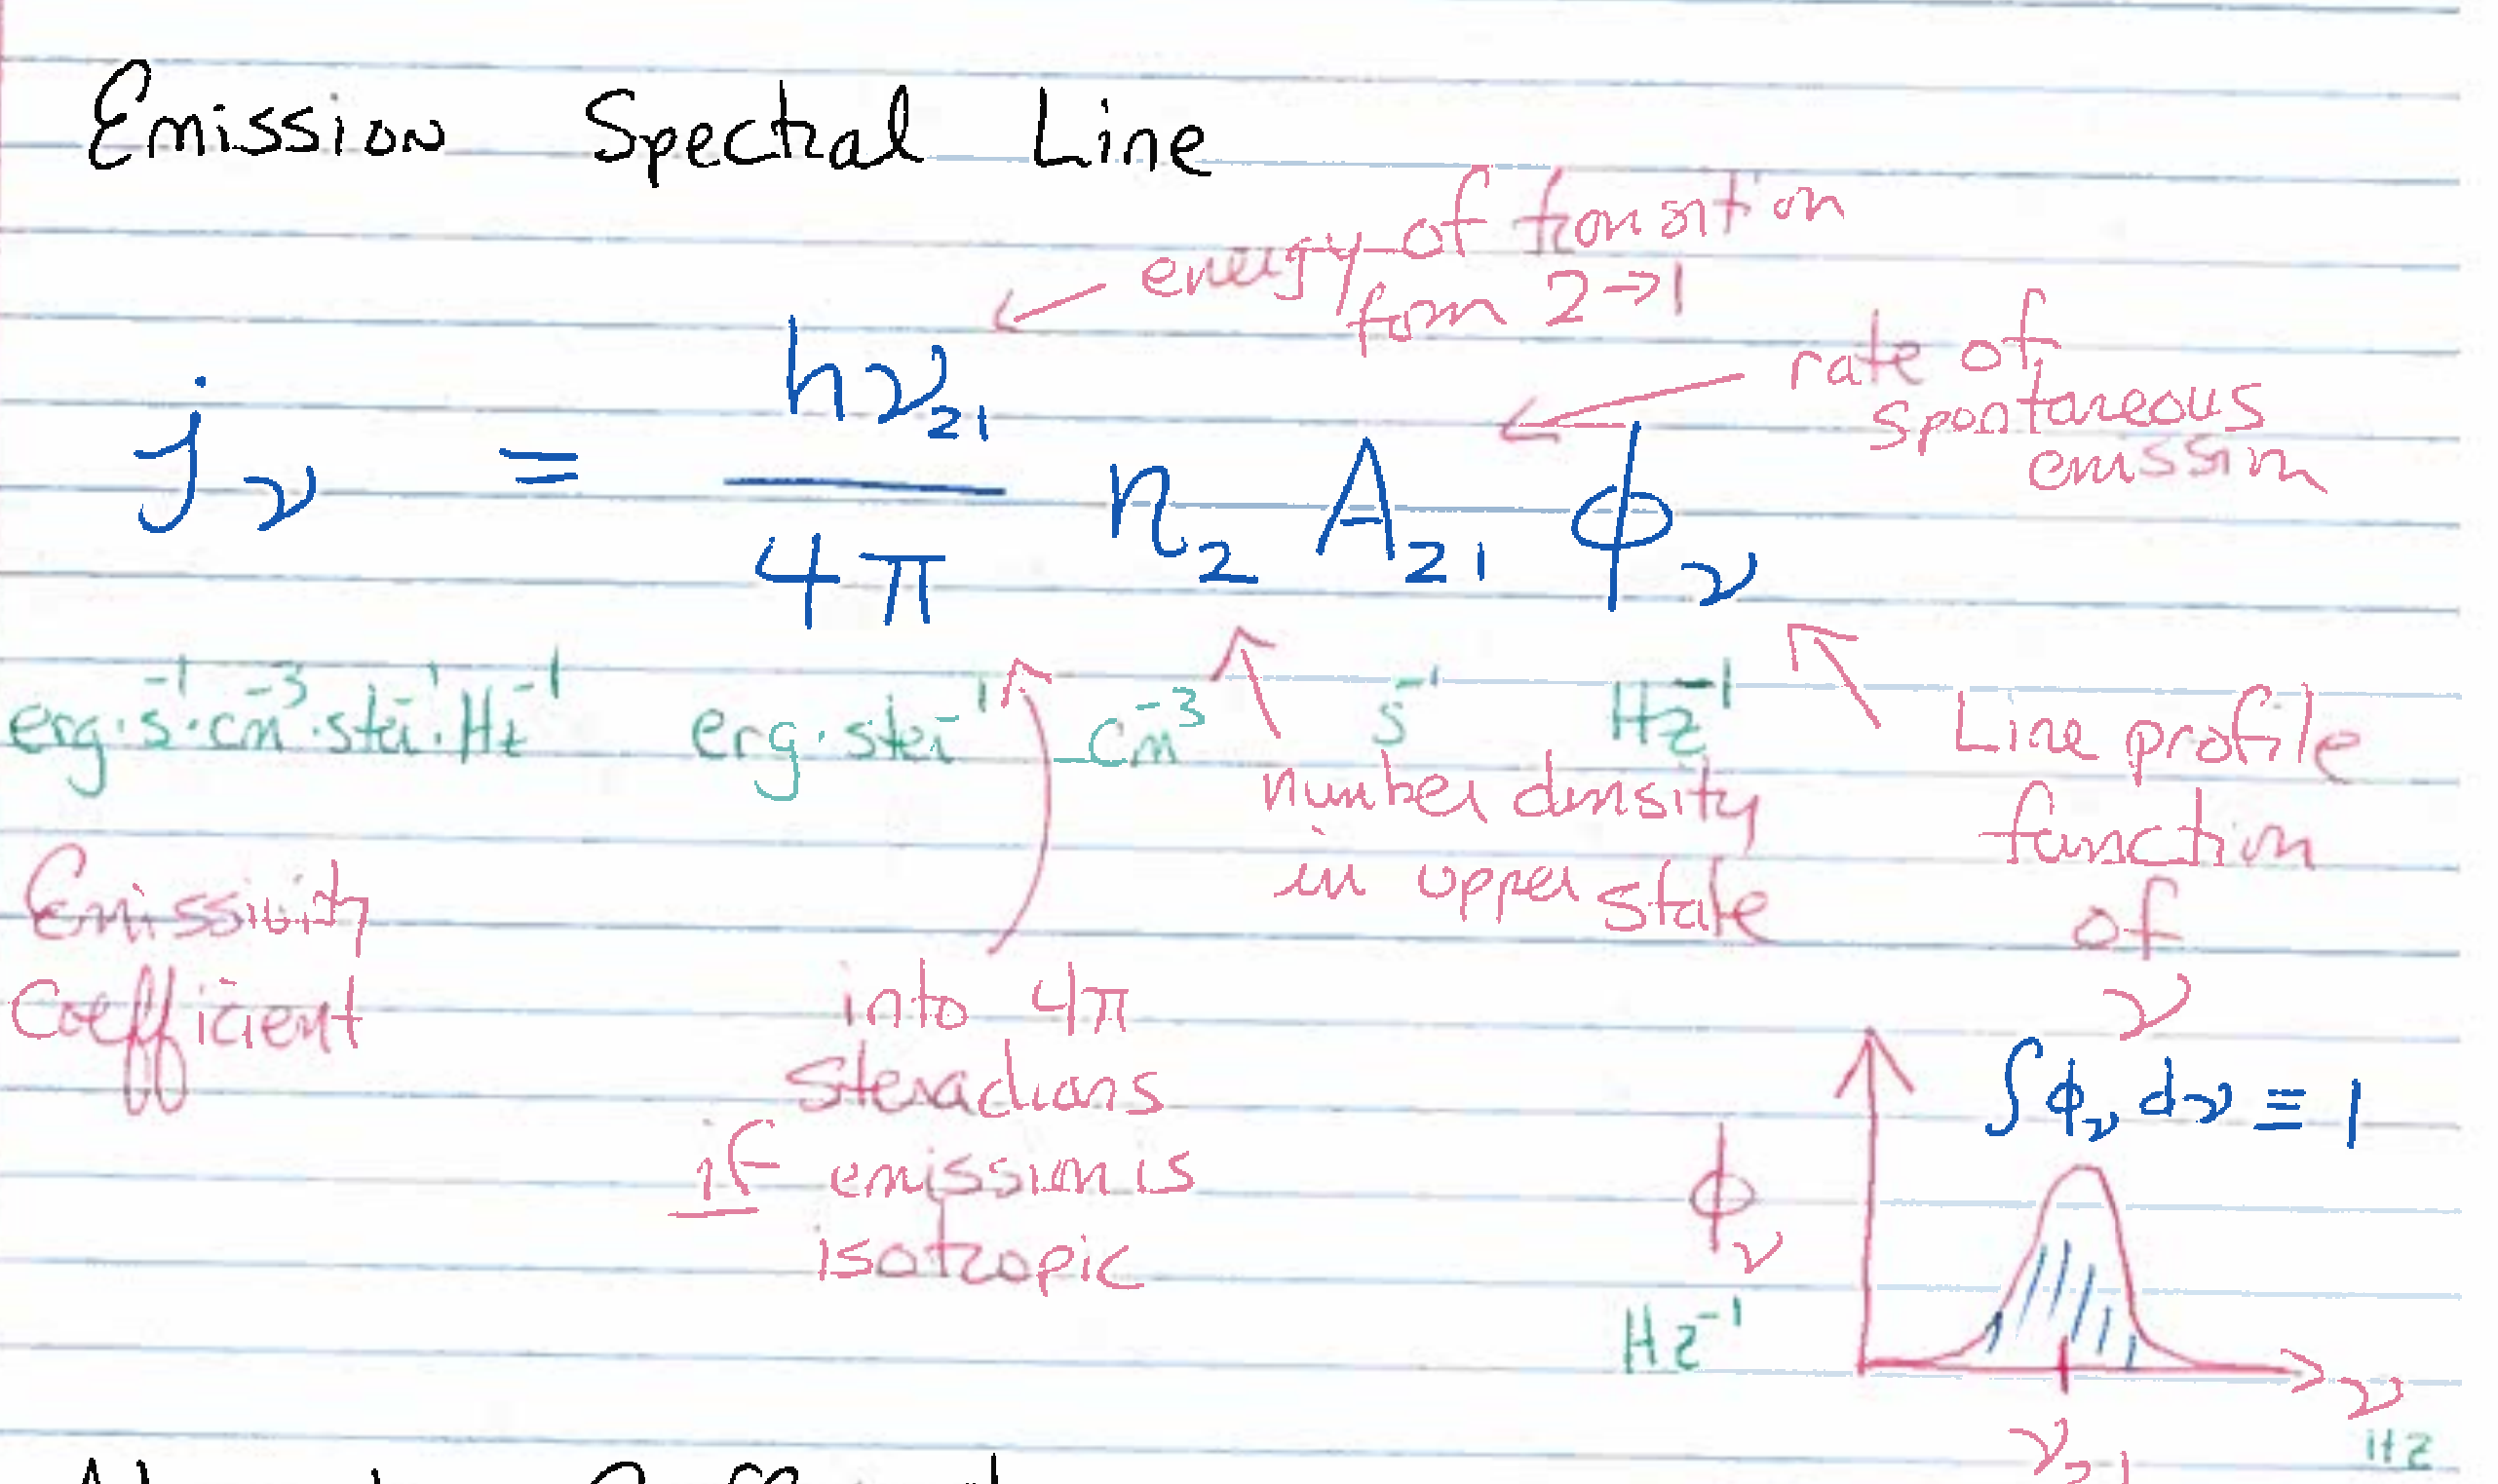
\includegraphics[scale=.5]{emission.png}

\subsection{Spontaneous Emission}

Spontaneous emission is the processes in which a atom/molecule transitions from an excited energy state to a lower energy state, emitting a photon. 
\\$\chi_\nu \longrightarrow h\nu + \chi_l$

When studying radiative processes, we usually use the emission coefficient $j_\nu$ to include in the equation the gain in intensity due to this emission. Then we have:

$j_\nu = \frac{dE}{dV d\Omega dt d\nu}$

$j_\nu = \frac{dI_\nu}{dS}$

$[j_\nu] = erg s^{-1} cm^{-2} str^{-1} Hz^{-1}$

\subsection{Stimulated Emission}

Stimulated emission is when an incoming photon interacts with an atomic electron and makes it drop to a lower energy level. The energy that this process releases goes to the electromagnetic field, creating a new photon with all the same properties as the previously incoming photon. Spontaneous emission is different because it does not relate to the electromagnetic field.

$\chi_\nu + h\nu \longrightarrow \chi_l + 2h\nu$

\subsection{Absorption}

Absorption is the processes in which a atom/molecule gets excited by an incoming photon and transitions from a lower energy state to a more energetic one.

$\chi_l + h\nu \longrightarrow \chi$

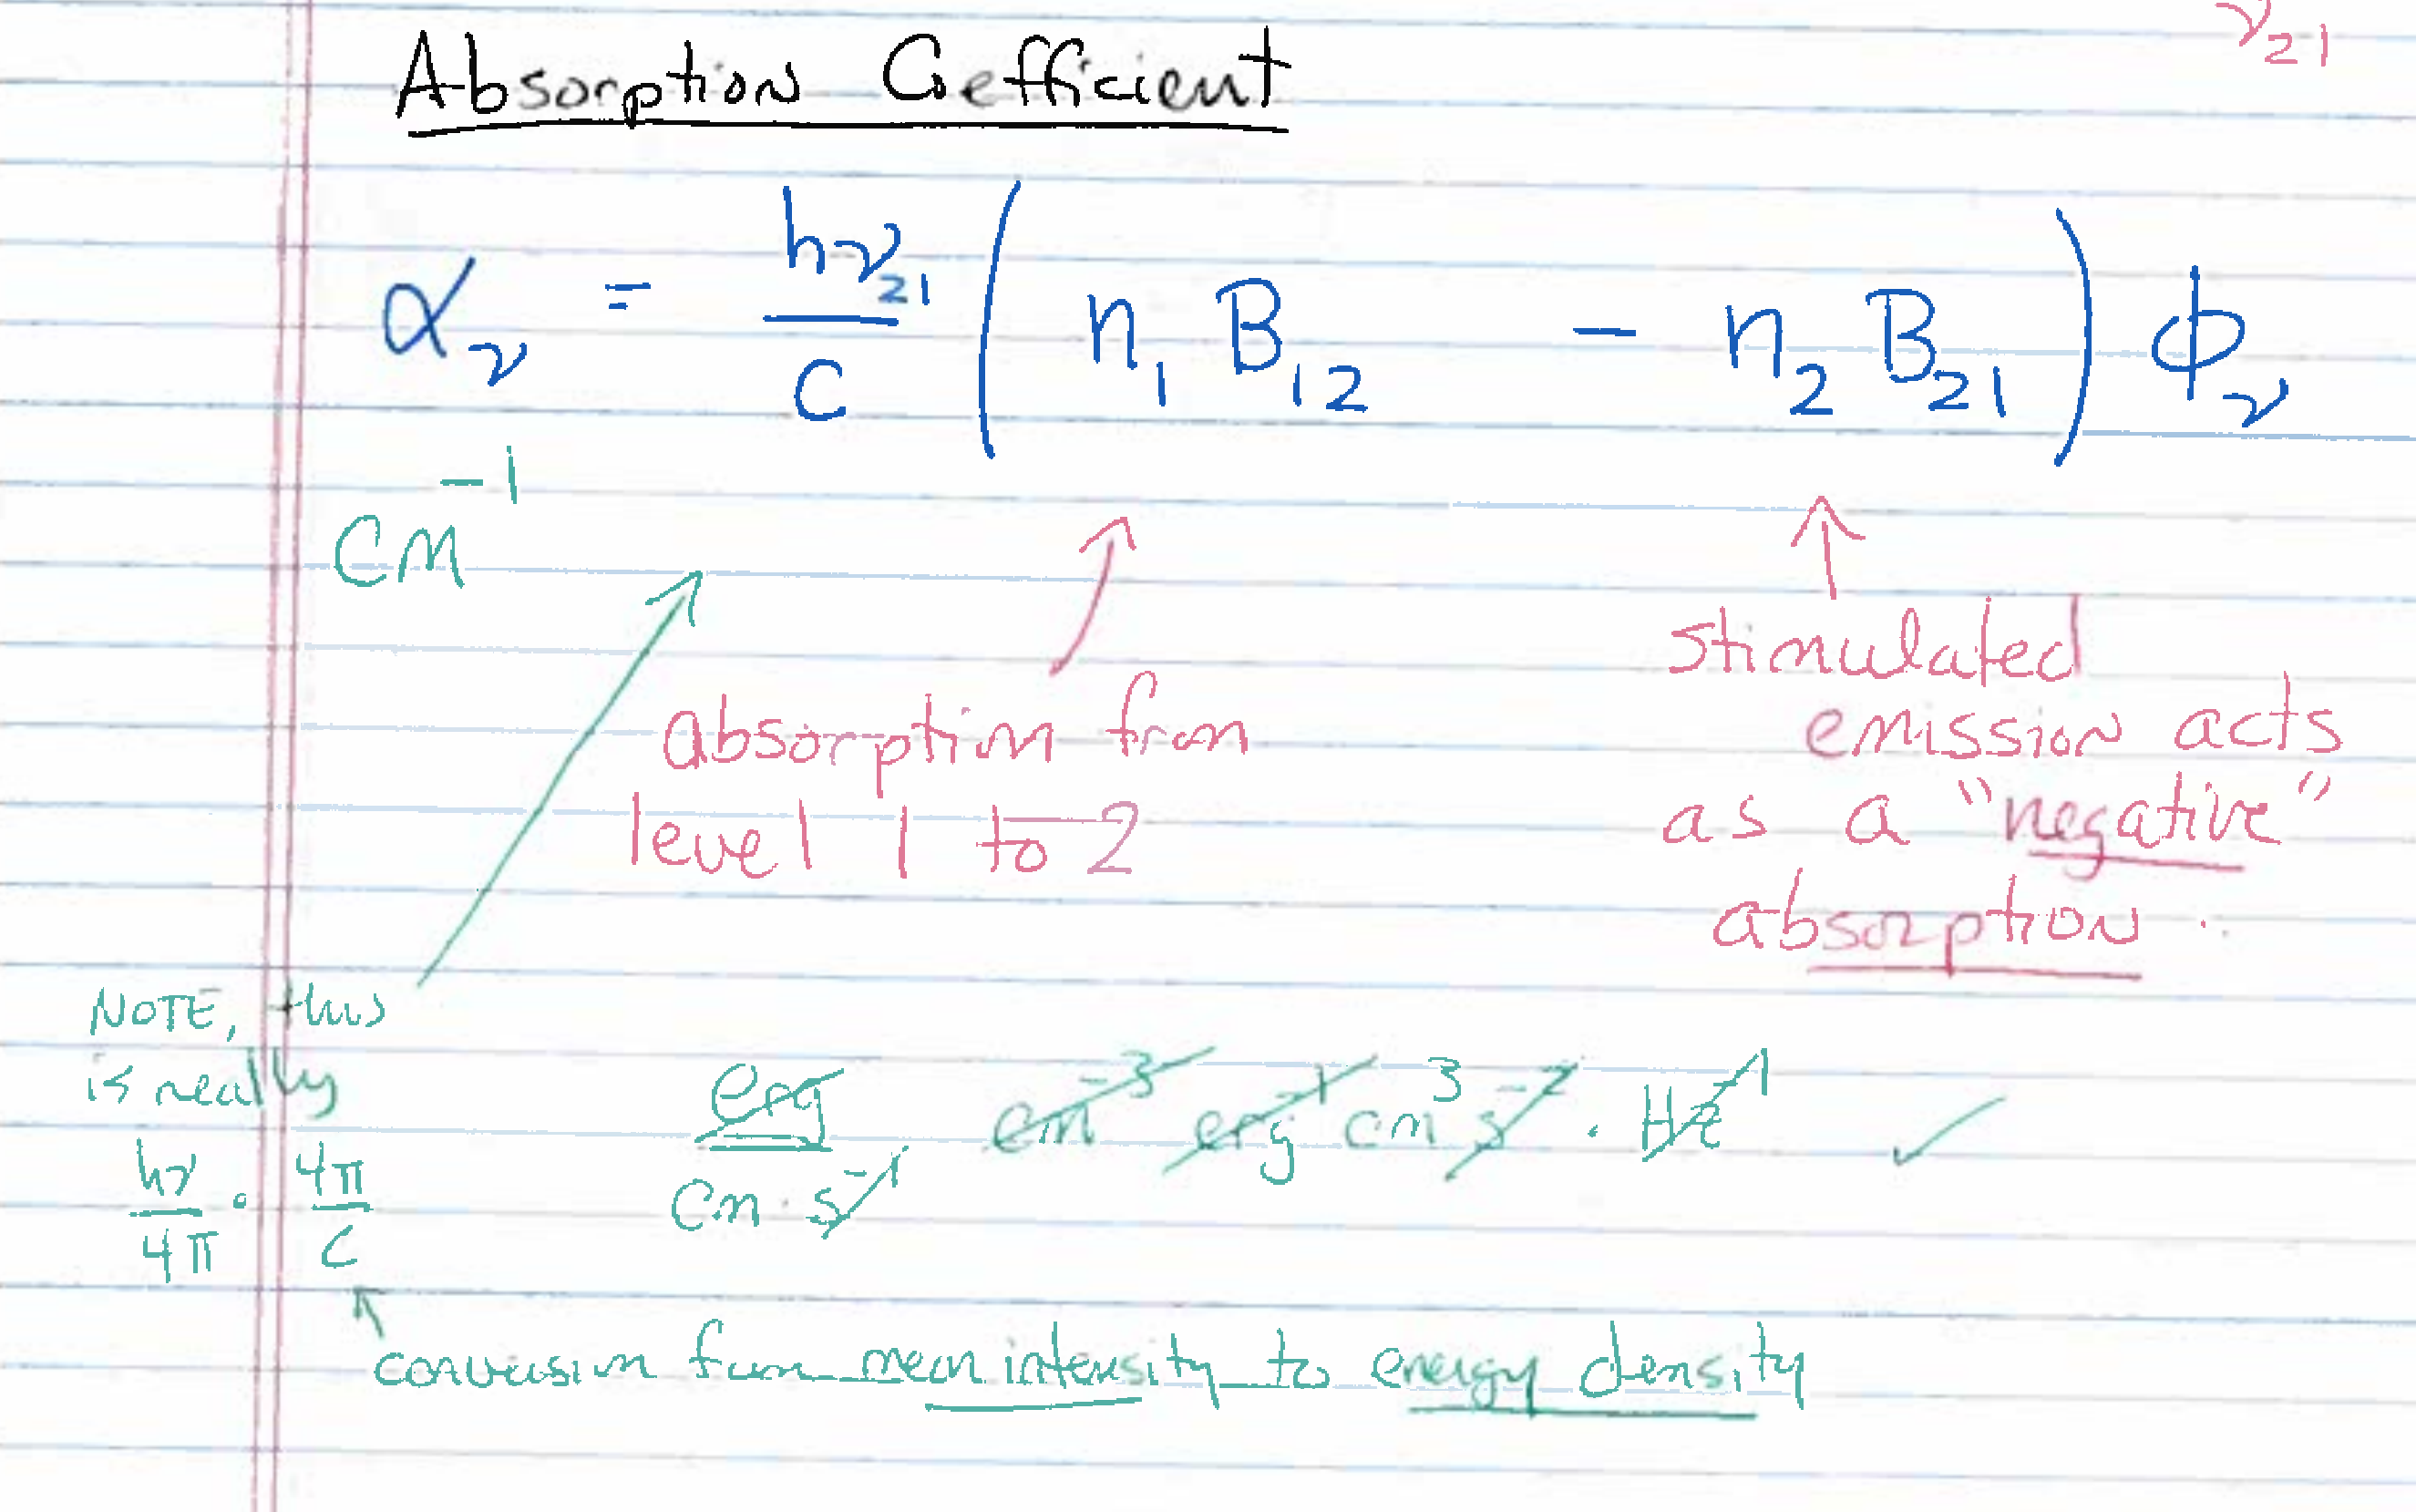
\includegraphics[scale=.5]{absorption.png}

\section{Absorption Cross-Section}
The relation between the monochromatic absorption cross section and a normalized
line profile $\phi_\nu$.
$\sigma_{lu}(\nu) = \frac{g_u}{g_l}\frac{c^2}{8\pi\nu^2_{lu}} A_{ul}\phi_\nu$
with
$\int \phi_\nu dv = 1.$

\section{Line Broadening Mechanisms}

    \subsection{Natrual Line Width}
    
        Lorentz Profile (Cauchy distribution):
        
        $ \phi_{\nu} = \frac{4 \gamma_{\rm UL}}{16 \pi^2 (\nu - \nu_{\rm UL})^2 + \gamma_{\rm UL}^2}$
        
        $\gamma = \sum_{Ej < Eu} A_{\rm uj} + \sum_{Ej > Ei} A_{\rm ij}$
        
        FWHM $ = \frac{\gamma_{\rm UL}}{2 \pi}$
        
        $\Delta v = \frac{c \Delta \nu}{\nu_{\rm UL}} = \frac{\gamma_{\rm UL} \lambda_{\rm UL}}{2 \pi} $
    
    \subsection{Doppler Broadening Profile}
    
        Gaussian Profile:
        
        $P_{\Vec{v}} = \frac{1}{\sqrt{2 \pi}} \frac{1}{\sigma_{\Vec{v}}} 
            e^{-(\Vec{v} - v_{\rm 0})^2 / 2 \sigma^2} $ 
            
        Here $\Vec{v}$ is the velocity and $\sigma$ is the 1D velocity dispersion.
        
    \subsection{Line Profile}\label{sec:line_profile}
    
        The line profile function can be thought of as "A probability function where a photon was emitted and can be absorbed". There are profiles for emitters and absorbers that determine the frequencies at which each emits or absorbs.
    
        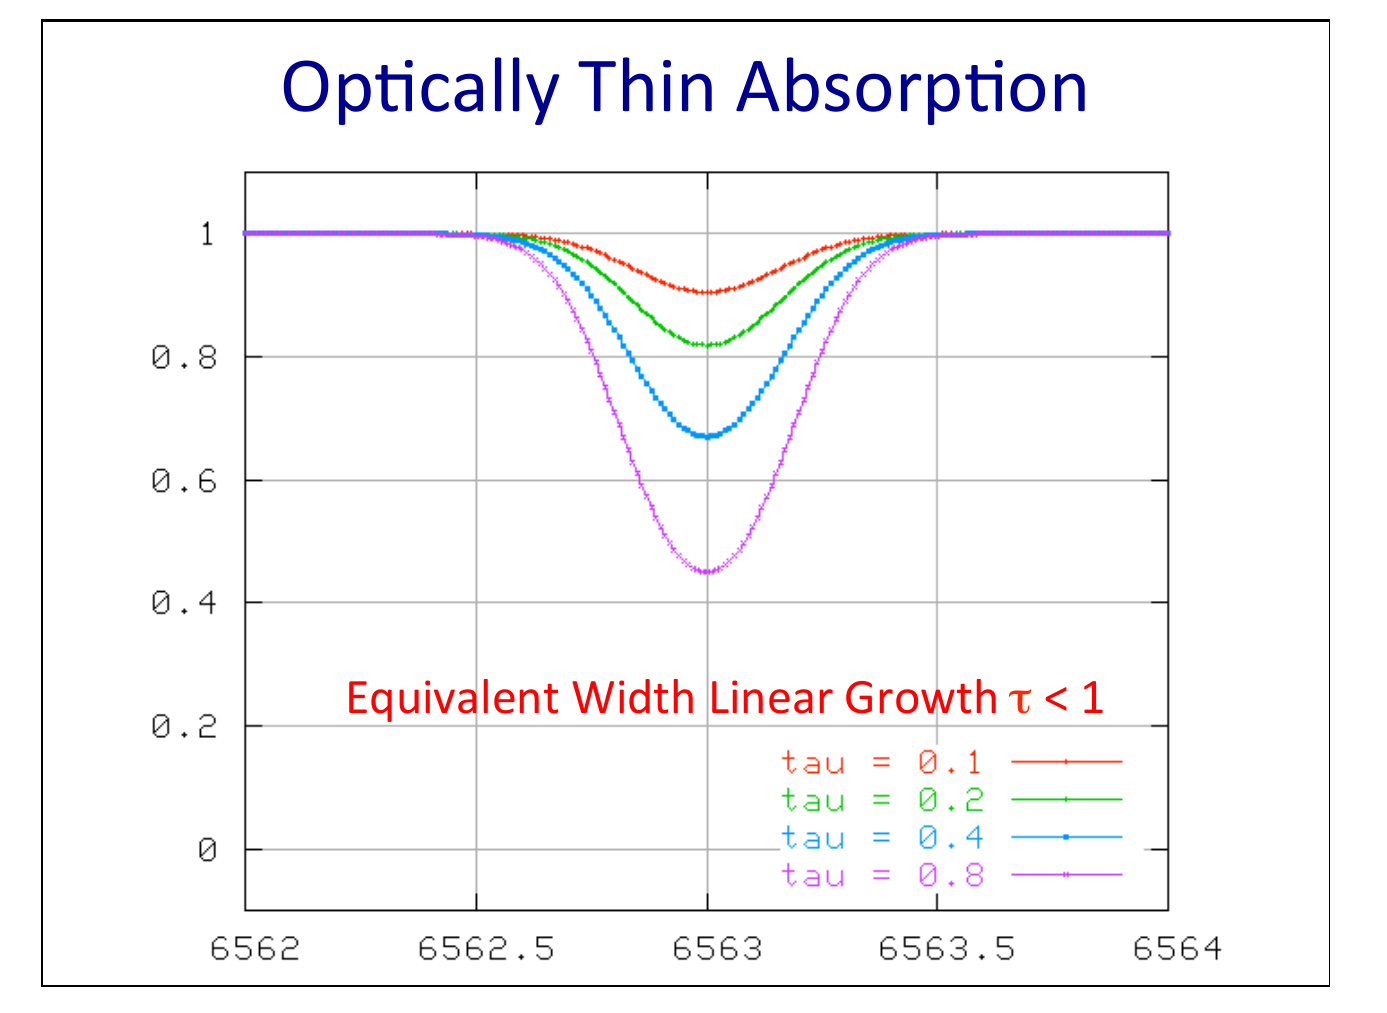
\includegraphics[scale=.5]{thin.png}
        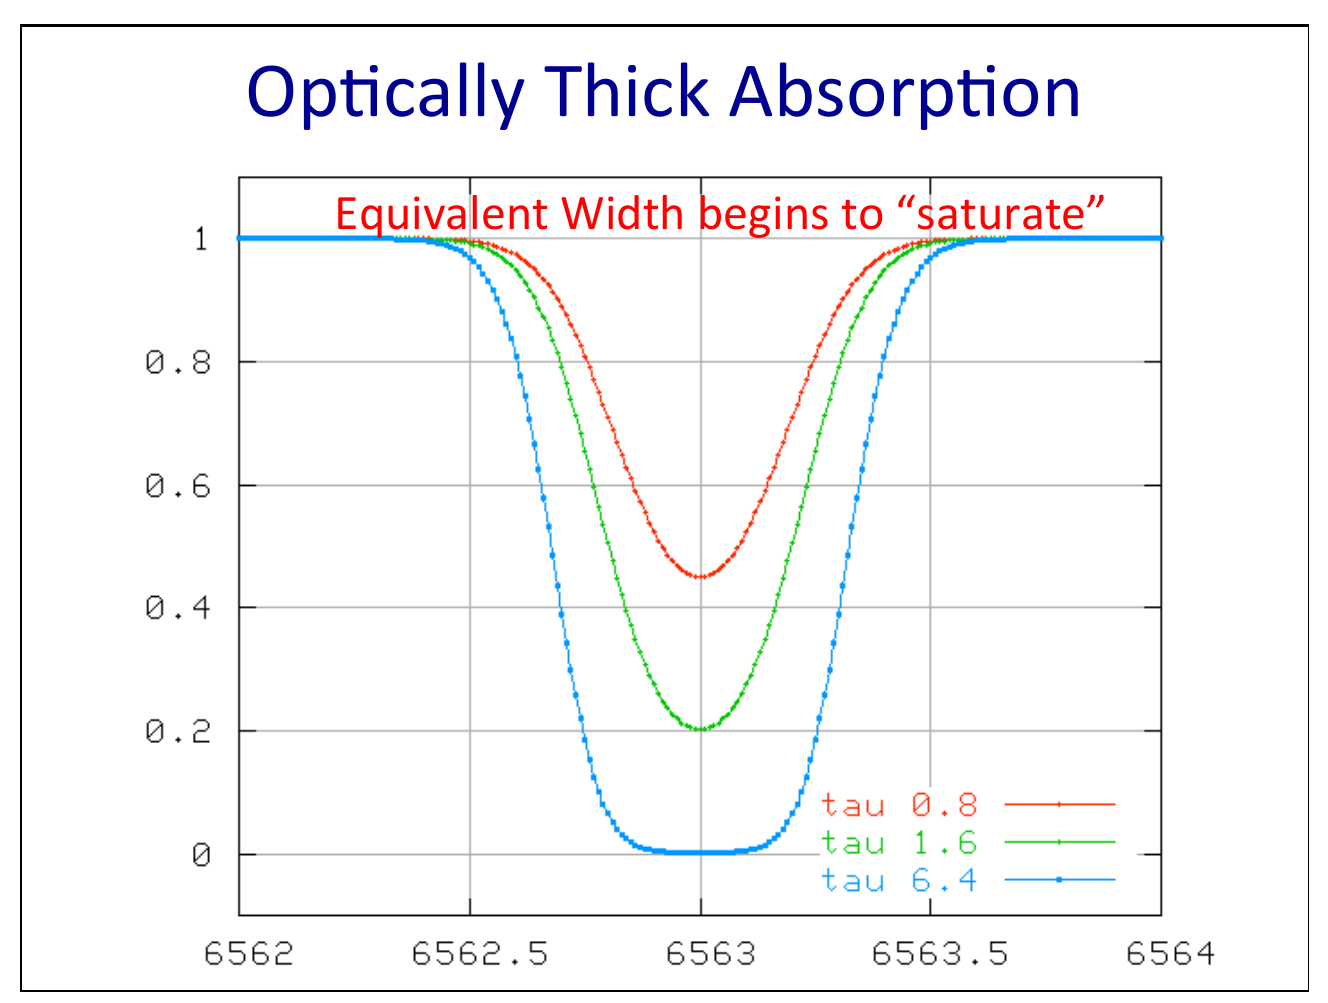
\includegraphics[scale=.5]{thick.png}
        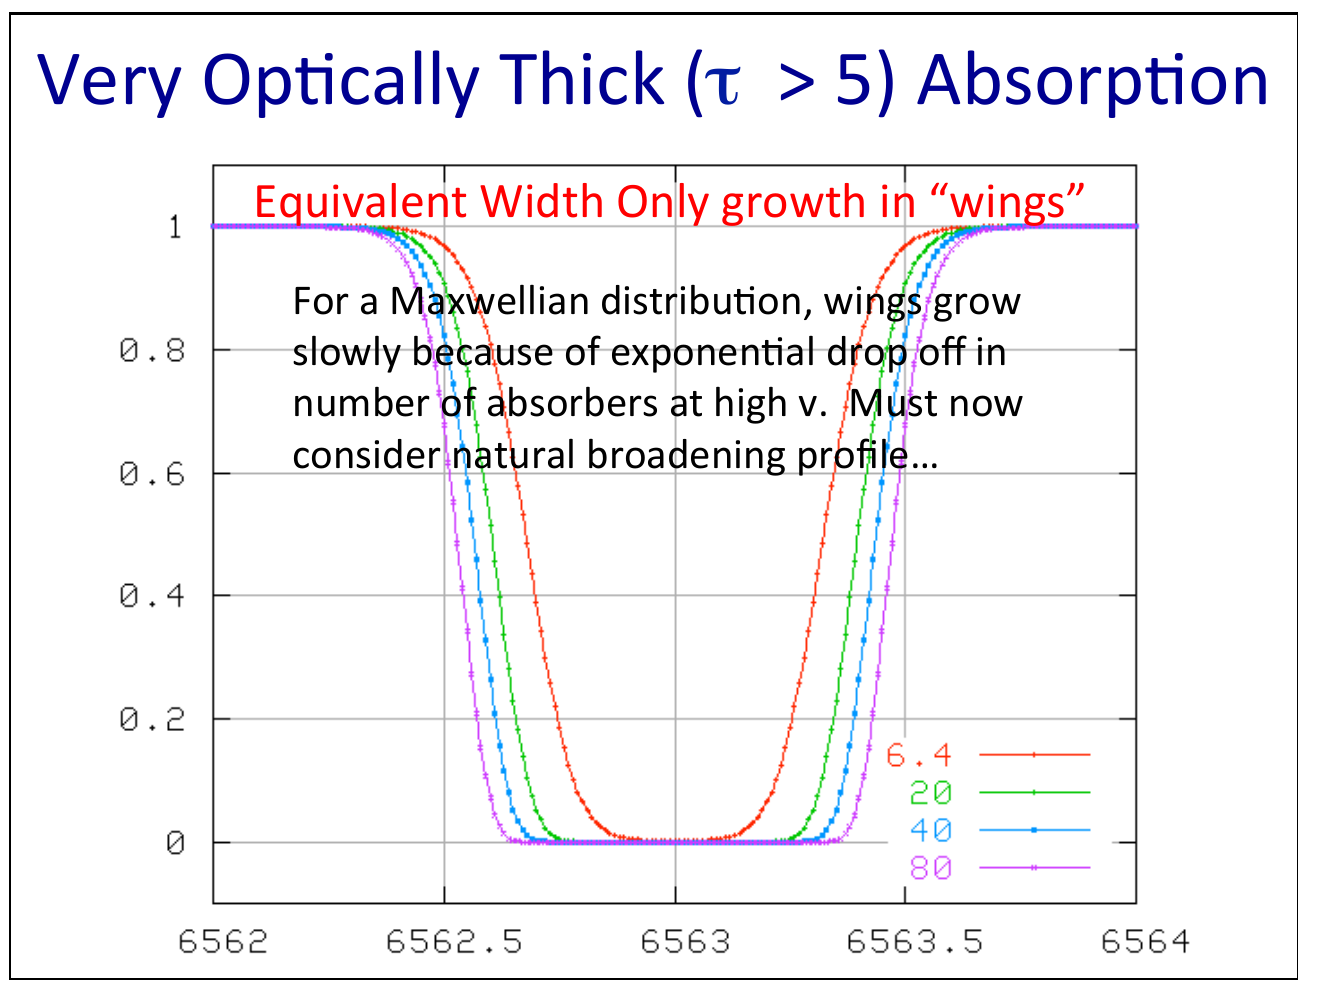
\includegraphics[scale=.5]{very_thick.png}

        The convolved line profile for both kinds of broadening effects:
        
        $ \phi = \int dv \; P_{\Vec{v}}(\Vec{v}) \frac{4 \gamma_{\rm UL}}{16 \pi^2 [\nu - (1-\nu) / (c \nu_{\rm UL}^2) ] + \gamma_{\rm UL}^2}$
